\documentclass[14pt]{extbook}
\usepackage{multicol, enumerate, enumitem, hyperref, color, soul, setspace, parskip, fancyhdr} %General Packages
\usepackage{amssymb, amsthm, amsmath, latexsym, units, mathtools} %Math Packages
\everymath{\displaystyle} %All math in Display Style
% Packages with additional options
\usepackage[headsep=0.5cm,headheight=12pt, left=1 in,right= 1 in,top= 1 in,bottom= 1 in]{geometry}
\usepackage[usenames,dvipsnames]{xcolor}
\usepackage{dashrule}  % Package to use the command below to create lines between items
\newcommand{\litem}[1]{\item#1\hspace*{-1cm}\rule{\textwidth}{0.4pt}}
\pagestyle{fancy}
\lhead{Progress Quiz 10}
\chead{}
\rhead{Version A}
\lfoot{1995-1928}
\cfoot{}
\rfoot{test}
\begin{document}

\begin{enumerate}
\litem{
Solve the equation below. Then, choose the interval that contains the solution.\[ -15(16x -11) = -13(-17x + 2) \]\begin{enumerate}[label=\Alph*.]
\item \( x \in [7.25, 7.55] \)
\item \( x \in [0.38, 0.47] \)
\item \( x \in [-0.32, -0.28] \)
\item \( x \in [0.11, 0.37] \)
\item \( \text{There are no real solutions.} \)

\end{enumerate} }
\litem{
Solve the linear equation below. Then, choose the interval that contains the solution.\[ \frac{9x -7}{4} - \frac{9x -4}{7} = \frac{4x + 5}{5} \]\begin{enumerate}[label=\Alph*.]
\item \( x \in [-2.54, 2.46] \)
\item \( x \in [18.22, 23.22] \)
\item \( x \in [13.26, 14.26] \)
\item \( x \in [44.7, 50.7] \)
\item \( \text{There are no real solutions.} \)

\end{enumerate} }
\litem{
Find the equation of the line described below. Write the linear equation as $ y=mx+b $ and choose the intervals that contain $m$ and $b$.\[ \text{Parallel to } 5 x + 8 y = 8 \text{ and passing through the point } (10, -10). \]\begin{enumerate}[label=\Alph*.]
\item \( m \in [-3.4, -1.5] \hspace*{3mm} b \in [-5.75, 0.25] \)
\item \( m \in [-0.9, -0.1] \hspace*{3mm} b \in [-5.75, 0.25] \)
\item \( m \in [-0.9, -0.1] \hspace*{3mm} b \in [-23, -19] \)
\item \( m \in [-0.9, -0.1] \hspace*{3mm} b \in [0.75, 6.75] \)
\item \( m \in [-0.6, 2.2] \hspace*{3mm} b \in [-16.25, -15.25] \)

\end{enumerate} }
\litem{
First, find the equation of the line containing the two points below. Then, write the equation as $ y=mx+b $ and choose the intervals that contain $m$ and $b$.\[ (-5, 4) \text{ and } (-11, -10) \]\begin{enumerate}[label=\Alph*.]
\item \( m \in [2.33, 7.33] \hspace*{3mm} b \in [9.67, 16.67] \)
\item \( m \in [2.33, 7.33] \hspace*{3mm} b \in [-3, 5] \)
\item \( m \in [-7.33, -1.33] \hspace*{3mm} b \in [-36.67, -34.67] \)
\item \( m \in [2.33, 7.33] \hspace*{3mm} b \in [-20.67, -13.67] \)
\item \( m \in [2.33, 7.33] \hspace*{3mm} b \in [7, 13] \)

\end{enumerate} }
\litem{
First, find the equation of the line containing the two points below. Then, write the equation as $ y=mx+b $ and choose the intervals that contain $m$ and $b$.\[ (7, 10) \text{ and } (5, 4) \]\begin{enumerate}[label=\Alph*.]
\item \( m \in [-1, 7] \hspace*{3mm} b \in [-16, -9] \)
\item \( m \in [-1, 7] \hspace*{3mm} b \in [6, 13] \)
\item \( m \in [-10, 0] \hspace*{3mm} b \in [19, 20] \)
\item \( m \in [-1, 7] \hspace*{3mm} b \in [-2, 0] \)
\item \( m \in [-1, 7] \hspace*{3mm} b \in [3, 6] \)

\end{enumerate} }
\litem{
Write the equation of the line in the graph below in Standard form $Ax+By=C$. Then, choose the intervals that contain $A, B, \text{ and } C$.
\begin{center}
    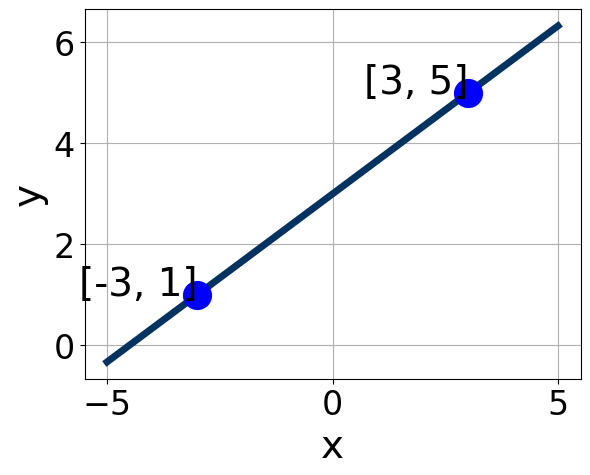
\includegraphics[width=0.5\textwidth]{../Figures/linearGraphToStandardA.png}
\end{center}
\begin{enumerate}[label=\Alph*.]
\item \( A \in [0.1, 4.2], \hspace{3mm} B \in [-0.55, 2.5], \text{ and } \hspace{3mm} C \in [-0.56, 1.91] \)
\item \( A \in [-5.5, -4.5], \hspace{3mm} B \in [-4.02, -1.97], \text{ and } \hspace{3mm} C \in [-3.6, -2.44] \)
\item \( A \in [0.1, 4.2], \hspace{3mm} B \in [-2.11, -0.52], \text{ and } \hspace{3mm} C \in [-1.04, 0.33] \)
\item \( A \in [3.3, 6.5], \hspace{3mm} B \in [-4.02, -1.97], \text{ and } \hspace{3mm} C \in [-3.6, -2.44] \)
\item \( A \in [3.3, 6.5], \hspace{3mm} B \in [2.26, 3.65], \text{ and } \hspace{3mm} C \in [2.89, 4.33] \)

\end{enumerate} }
\litem{
Solve the linear equation below. Then, choose the interval that contains the solution.\[ \frac{8x + 5}{8} - \frac{3x -7}{3} = \frac{9x -9}{4} \]\begin{enumerate}[label=\Alph*.]
\item \( x \in [0.6, 2.1] \)
\item \( x \in [2.2, 3.4] \)
\item \( x \in [8.5, 10.6] \)
\item \( x \in [-1.2, 0.9] \)
\item \( \text{There are no real solutions.} \)

\end{enumerate} }
\litem{
Write the equation of the line in the graph below in Standard form $Ax+By=C$. Then, choose the intervals that contain $A, B, \text{ and } C$.
\begin{center}
    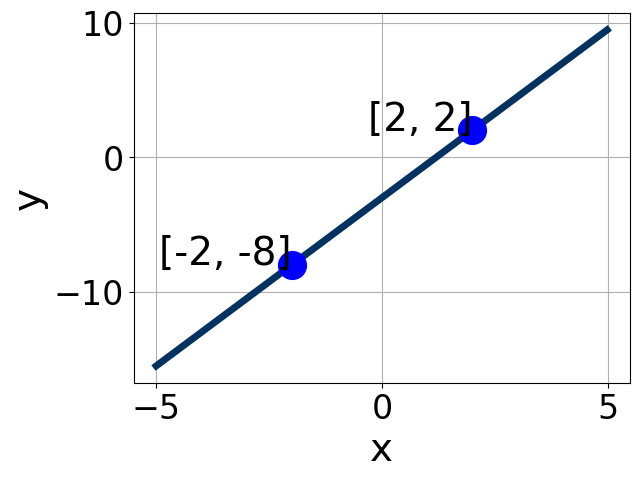
\includegraphics[width=0.5\textwidth]{../Figures/linearGraphToStandardCopyA.png}
\end{center}
\begin{enumerate}[label=\Alph*.]
\item \( A \in [-3.93, -1.25], \hspace{3mm} B \in [-3.26, -1.3], \text{ and } \hspace{3mm} C \in [10, 12] \)
\item \( A \in [0.96, 1.65], \hspace{3mm} B \in [-1.16, -0.92], \text{ and } \hspace{3mm} C \in [4, 9] \)
\item \( A \in [2.11, 4.08], \hspace{3mm} B \in [-3.26, -1.3], \text{ and } \hspace{3mm} C \in [10, 12] \)
\item \( A \in [2.11, 4.08], \hspace{3mm} B \in [1.93, 2.42], \text{ and } \hspace{3mm} C \in [-17, -6] \)
\item \( A \in [0.96, 1.65], \hspace{3mm} B \in [0.85, 1.42], \text{ and } \hspace{3mm} C \in [-6, 1] \)

\end{enumerate} }
\litem{
Find the equation of the line described below. Write the linear equation as $ y=mx+b $ and choose the intervals that contain $m$ and $b$.\[ \text{Perpendicular to } 3 x + 8 y = 12 \text{ and passing through the point } (2, 10). \]\begin{enumerate}[label=\Alph*.]
\item \( m \in [0.67, 4.67] \hspace*{3mm} b \in [-4.67, 2.33] \)
\item \( m \in [0.67, 4.67] \hspace*{3mm} b \in [6, 9] \)
\item \( m \in [-2.62, 1.38] \hspace*{3mm} b \in [3.67, 5.67] \)
\item \( m \in [0.67, 4.67] \hspace*{3mm} b \in [3.67, 5.67] \)
\item \( m \in [-4.67, -1.67] \hspace*{3mm} b \in [15.33, 18.33] \)

\end{enumerate} }
\litem{
Solve the equation below. Then, choose the interval that contains the solution.\[ -18(-16x -14) = -7(-13x + 12) \]\begin{enumerate}[label=\Alph*.]
\item \( x \in [-1.95, -1.04] \)
\item \( x \in [-1.4, -0.68] \)
\item \( x \in [0.45, 0.88] \)
\item \( x \in [-0.65, -0.29] \)
\item \( \text{There are no real solutions.} \)

\end{enumerate} }
\end{enumerate}

\end{document}